\chapter{On Mobile Analytics}
Mobile Analytics, an umbrella term that encompasses various aspects of:
\begin{itemize}
    \item Products and/or Services:
    \item Software libraries:
    \item Data reporting, filtering, collection, propagation, import, storage, analysis, reporting, export
    \item Data use and ownership, data 'protection', privacy, sensitive data, permissions, etc.
    \item Types and extent of data collected, and not collected (which affects the ability to analyse, fault-find, etc.)
    \item The history and movements in the industry might also be relevant and of interest.
\end{itemize}

Include my 3 layers figure. Perhaps the 3 views of quality figure. My data sources figure. 

\section{Layers of an app}
\begin{enumerate}
    \item User Interface:
    \item The rest of the app:
    \item The platform's perspective of an app:
\end{enumerate}

\subsection{Mapping Analytics tools to layers of an app}

\subsection{Key components of Mobile Analytics}
\begin{itemize}
    \item [Local] Logging component, on device:
    \item Software that records pertinent data locally:
    \item Local data collector:
    \item Data transmitter:
    \item A Conduit:
    \item Data receiver:
    \item Load, validate, transform:
    \item Data base:
    \item Data processing (e.g. filtering, grouping and aggregation, pattern recognition and matching, etc.)
    \item Report Generator:
    \item User Interfaces, including APIs:
\end{itemize}

\subsubsection{Four perspectives on mobile apps}
\large{\texttt{\emph{1} Public \textbf{(}\emph{2} User \textbf{(}\emph{3} Development team \textbf{(}\emph{4} App Store\textbf{)))}}}

App stores have established various groups of people, each has a distinct view of the mobile apps in the app store. Broadly, the public (group 1) knows the least, and the app store (group 4) knows the most.

Groups and their perspectives:
\begin{enumerate}
    \item \textbf{Public}: The public can see information that is publicly available in the app store pertaining to apps. This information includes screenshots, descriptions, popularity, and additional information about particular apps. They may also see rankings, promoted apps, etc.
    \item \textbf{User}: A user has installed an app, they can explore the app and use it. They may form opinions on the usefulness, value and quality of the app. They determine whether they use it, and when. They may stop using it for whatever reason, and may uninstall the app. QoE and UX both pertain to user's and their perspectives of an app.
    \item \textbf{Development team}: The development team own the creation and development of an app. They may also maintain and support it. They may obtain information from various sources pertaining to the use of their app from their app's user-base. They choose what an app reports and to whom in terms of logging recorded by, and analytics sent by, the app.
    \item \textbf{App Store}: The app store has an aggregate perspective of all the apps in their app store (and also apps they have suspended or rejected).
\end{enumerate}

\begin{figure}[ht]
    \centering
    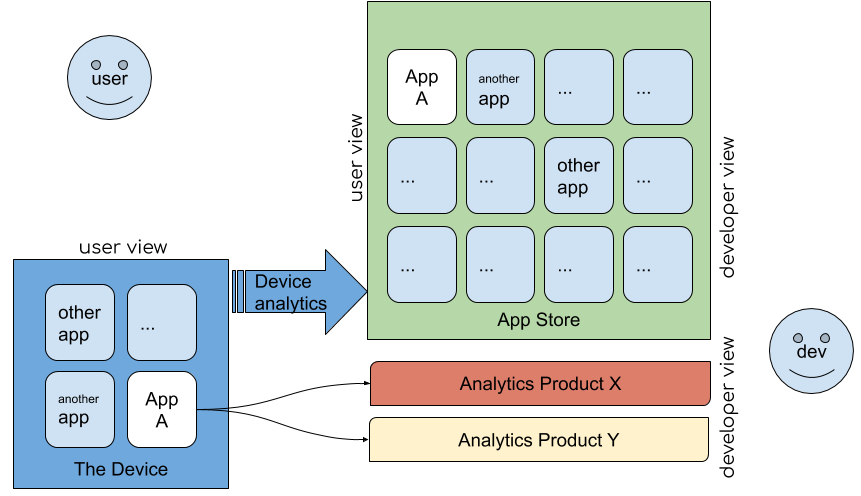
\includegraphics[width=\textwidth]{images/data_sources_and_views_25_jan_2020.jpg}
    \caption{Data sources and views}
    \label{fig:data_sources_and_views}
\end{figure}

Data can be collected by apps, devices, and the app store, as illustrated in Figure \ref{fig:data_sources_and_views}. Users can see which apps they have installed on their device and may be able to decide whether device analytics is collected. They can also see publicly available information about apps in the app store. Developers can see the same public data in the app store, they can also see additional data Google gathers and provides about \textit{their} apps together with whatever access they have to analytics tools incorporated into these apps.

Note: the third set of observers are the people and organisations who provide the app store and the various tools and products. They have a unique perspective across \textit{all the apps} that use their product. Google, for instance, calculates and publishes app-store wide "Bad behavior thresholds" for crash rates (1.09\%) and ANRs (0.47\%).

\section{Characteristics of Analytics Tools}


\begin{itemize}
    \item Status and Reporting of problems and outages
    \item Testability
    \item Performance Characteristics (Latency, Volumes,...)
    \item Time (Timezones, Daily Updates, Reporting periods, Data availability,...)
    \item Interoperability with external software e.g. for integration, analysis
    \item Vitality and Popularity: 
    \item Pricing:
    \item TBC
\end{itemize}
